\documentclass[11pt]{article}
\usepackage{subfigure,wrapfig,graphicx,booktabs,fancyhdr,amsmath,amsfonts,appendix,tikz}
\usepackage{bm,amssymb,amsthm,wasysym,color,fullpage,setspace,multirow,placeins}
\usepackage{pgfplots}
\pgfplotsset{compat=1.18}
\usepackage{amsmath,amssymb}
\usepackage{tcolorbox}

% Custom math commands
\newcommand{\vb}{\boldsymbol}
\newcommand{\vbh}[1]{\hat{\boldsymbol{#1}}}
\newcommand{\vbb}[1]{\bar{\boldsymbol{#1}}}
\newcommand{\vbt}[1]{\tilde{\boldsymbol{#1}}}
\newcommand{\vbs}[1]{{\boldsymbol{#1}}^*}
\newcommand{\vbd}[1]{\dot{{\boldsymbol{#1}}}}
\newcommand{\vbdd}[1]{\ddot{{\boldsymbol{#1}}}}
\newcommand{\by}{\times}
\newcommand{\tr}{{\rm tr}}
\newcommand{\cpe}[1]{\left[{#1} \times\right]}
\newcommand{\sfrac}[2]{\textstyle\frac{#1}{#2}}

% Title and Author Information
\title{Homework 5}
\author{Jacob Hands \\ COE 352}
\date{October 24, 2023}

\begin{document}
\maketitle

\section*{Problem 1}

\textbf{(20 pts)} Use a uniform four-element mesh on $[0, 1]$ and piecewise Lagrangian linear finite element basis functions to construct a finite element interpolant, \( f_h \), of the function \( f(x) = \sin(\pi x) \). Set the values \( f_h(x_i) = \sin(\pi x_i) \) for \( i = 1, 2, 3, 4, 5 \), and plot the function \( f \) and \( f_h \).

\section*{Solution}

Let the mesh points be \( x_0 = 0 \), \( x_1 = 0.25 \), \( x_2 = 0.5 \), \( x_3 = 0.75 \), and \( x_4 = 1 \). For each node, we compute:
\[
f_h(x_i) = f(x_i) = \sin(\pi x_i) \quad \text{for } i = 0, 1, 2, 3, 4.
\]
Using linear basis functions for each element, we can construct \( f_h(x) \) as a piecewise linear function interpolating these values. We then plot \( f(x) \) and \( f_h(x) \).

% Include your figure here for Problem 1
\begin{figure}[!h]
    \centering
    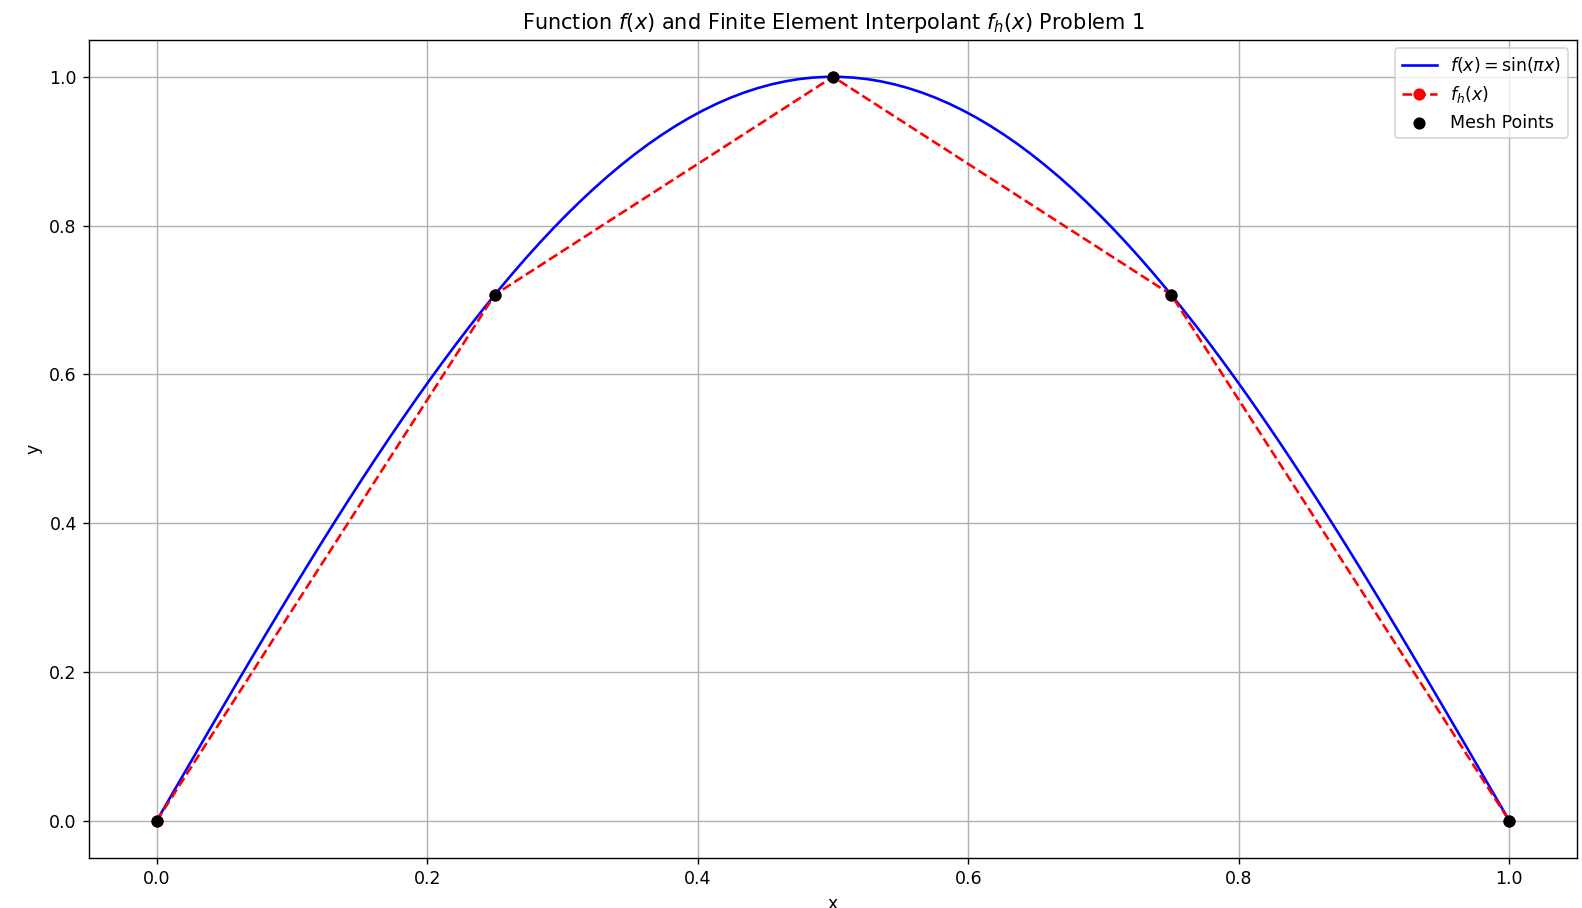
\includegraphics[width=0.7\textwidth]{images/problem1.png}
    \caption{Plot of $f(x) = \sin(\pi x)$ and finite element interpolant $f_h(x)$}
\end{figure}
\FloatBarrier

\newpage

\section*{Problem 2}

\textbf{Consider the boundary value problem}
\[
-y'' = x, \quad y(0) = y(1) = 0.
\]

\subsection*{(a) (10 pts) Find the exact solution of the problem.}

To find the exact solution, we solve:
\[
y'' = -x.
\]
Integrating twice, we get:
\[
y'(x) = -\frac{x^2}{2} + C_1,
\]
\[
y(x) = -\frac{x^3}{6} + C_1 x + C_2.
\]
Using the boundary conditions \( y(0) = 0 \) and \( y(1) = 0 \), we find:
\[
y(0) = C_2 = 0,
\]
\[
y(1) = -\frac{1}{6} + C_1 = 0 \Rightarrow C_1 = \frac{1}{6}.
\]
Thus, the exact solution is:
\[
y(x) = -\frac{x^3}{6} + \frac{x}{6}.
\]

\subsection*{(b) (10 pts) Derive the weak form of the problem.}

To derive the weak form, multiply both sides by a test function \( v(x) \) and integrate over \( [0, 1] \):
\[
\int_0^1 -y'' v \, dx = \int_0^1 x v \, dx.
\]
Integrating by parts, we get:
\[
\left. -y' v \right|_0^1 + \int_0^1 y' v' \, dx = \int_0^1 x v \, dx.
\]
Applying the boundary conditions \( y(0) = y(1) = 0 \), the weak form becomes:
\[
\int_0^1 y' v' \, dx = \int_0^1 x v \, dx.
\]

\subsection*{(c) (20 pts) Galerkin Approximation with Basis Functions}

Let \( N = 3 \) and choose basis functions \( \phi_i = \sin(i \pi x) \) for \( i = 1, 2, 3 \). The Galerkin method requires us to calculate the stiffness matrix \( K_{ij} \) and load vector \( f_i \).

1. **Stiffness Matrix**: 
   \[
   K_{ij} = \int_0^1 \phi_i' \phi_j' \, dx.
   \]
   From the calculations in the notes, we have for each entry:
   \[
   K_{ij} = \int_0^1 \left( i \pi \cos(i \pi x) \right) \left( j \pi \cos(j \pi x) \right) \, dx.
   \]
   Each entry \( K_{ij} \) is computed and substituted in the matrix.

2. **Load Vector**:
   \[
   f_i = \int_0^1 x \phi_i \, dx.
   \]
   Substitute each basis function \( \phi_i(x) = \sin(i \pi x) \), and evaluate each integral to find \( f_i \).

Solving the resulting system of equations for the coefficients gives the approximate solution \( y_h(x) \).


% Include your figure here for Problem 2 (exact and approximate solution plot)
\begin{figure}[!h]
    \centering
    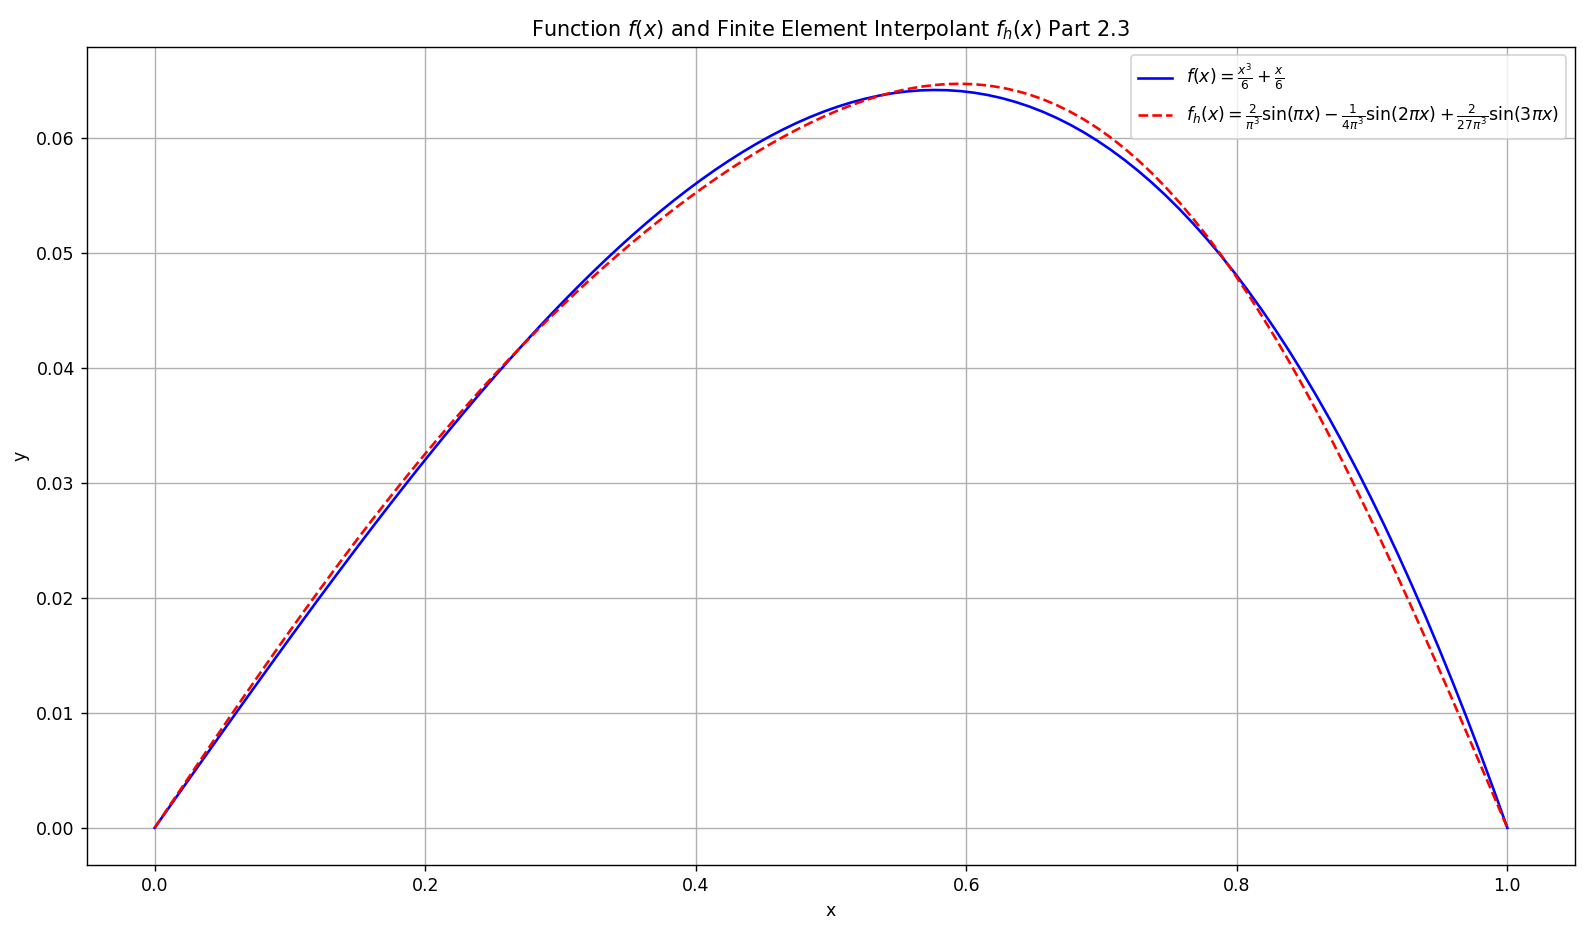
\includegraphics[width=0.7\textwidth]{images/problem2_3.png}
    \caption{Plot of exact solution $y(x)$ and approximate solution $y_h(x)$}
\end{figure}
\FloatBarrier
\subsection*{(d) (40 pts) Galerkin Piece-wise Linear Finite Element Approximation}

Using a uniform mesh with mesh size \( h = 0.25 \), we have nodes at \( x = 0, 0.25, 0.5, 0.75, 1 \). Define piecewise linear basis functions corresponding to each interval.

1. **Local Stiffness Matrix for Each Element**:
   For each element \( e \), the local stiffness matrix is:
   \[
   K_{ij}^e = \int_{x_e}^{x_{e+1}} \phi_i' \phi_j' \, dx 
   \]
   Summing these contributions forms the global stiffness matrix.

2. **Local Load Vector for Each Element**:
   For each element, compute:
   \[
   f_i^e = \int_{x_e}^{x_{e+1}} x \phi_i \, dx.
   \]
   This yields the components of the global load vector, which are then assembled from each element.

3. **Assemble the Global System**:
   Solve the resulting system to find the approximate solution \( y_h(x) \).

% Include your figure here for Problem 2d (exact and approximate solution plot with mesh size h=0.25)
\begin{figure}[!h]
    \centering
    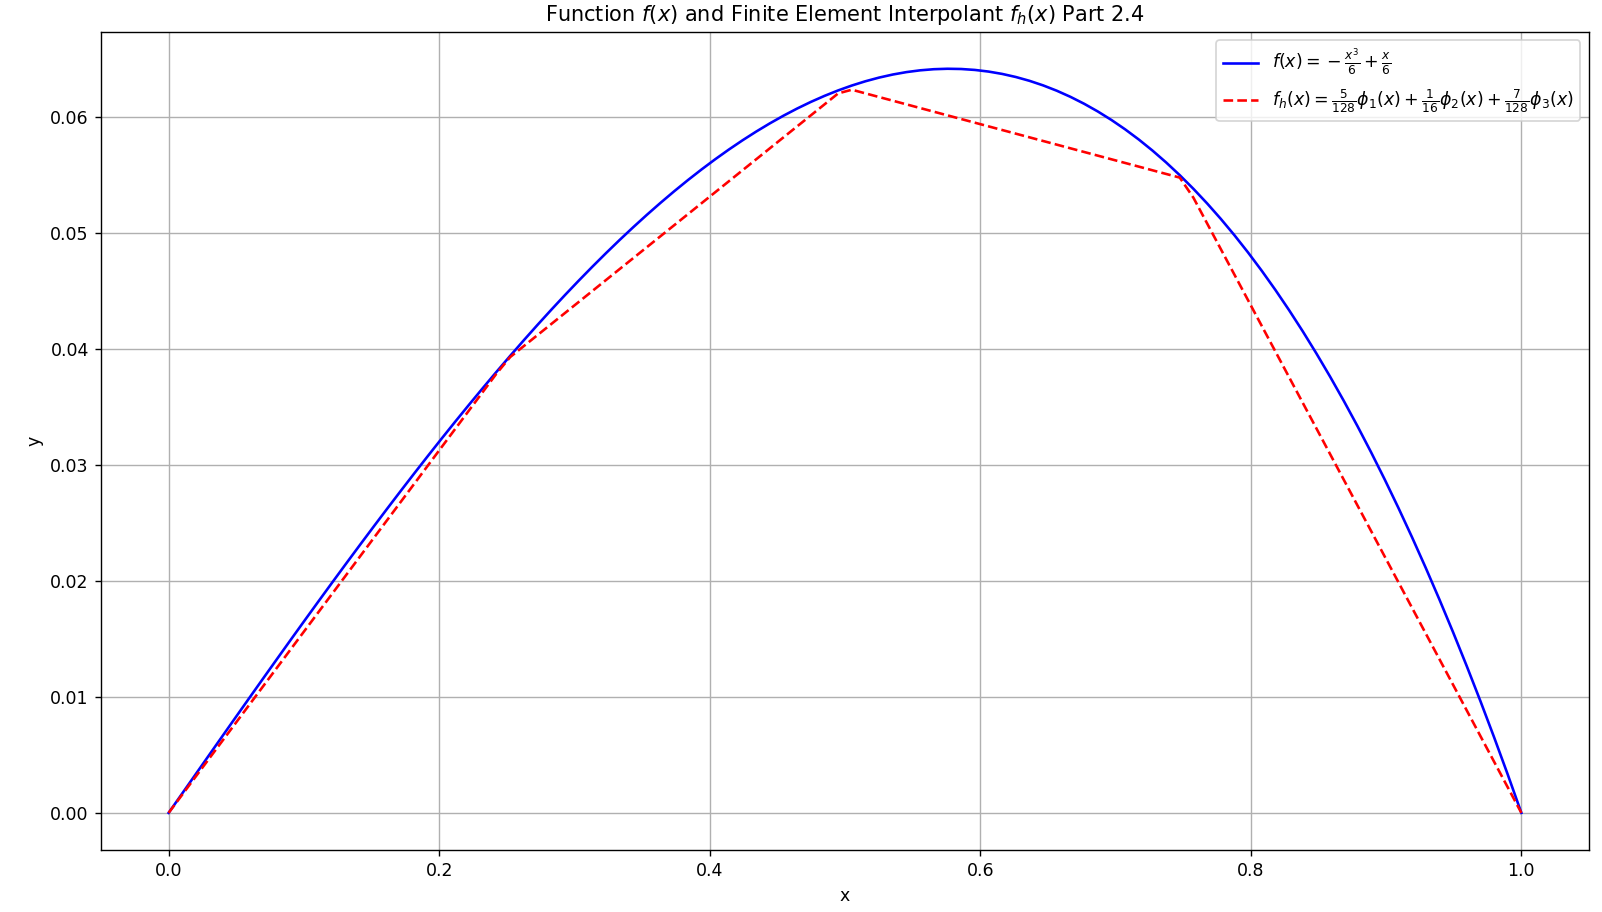
\includegraphics[width=0.7\textwidth]{images/problem2_4.png}
    \caption{Plot of exact solution $y(x)$ and finite element approximation $y_h(x)$ with $h=0.25$}
\end{figure}
\FloatBarrier

\end{document}
